% Section 4: Brinksmanship  
%------------------------------------------------------------------------------%

\begin{frame}{Brinksmanship}
  \begin{itemize}
    \item In the last lecture, we learned about different roles \alert{uncertainty} can play in games 
    \item In this lecture we are talking about manipulating the rules of a game
    \item The idea of \alert{brinksmanship} asks about when players might strategically implement uncertainty to their advantage
  \end{itemize} 
\end{frame}

\begin{frame}{Assignment 2 - Question 4}
  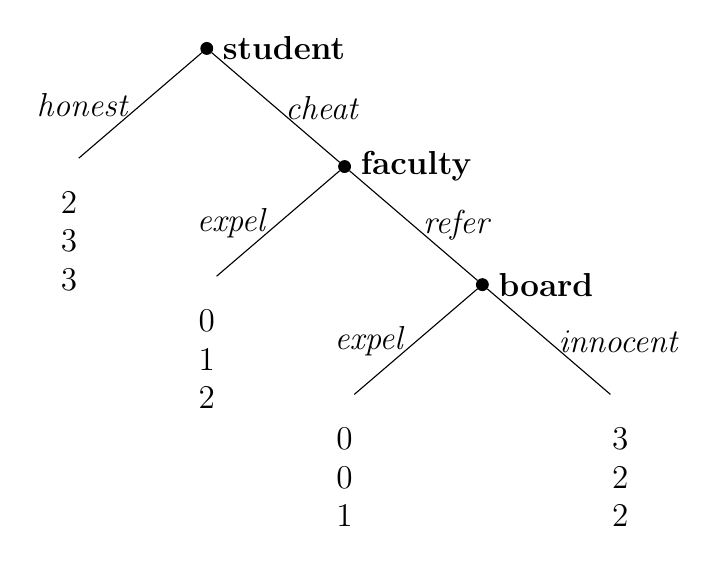
\begin{tikzpicture}[scale=1.0,font=\large]
  \tikzstyle{solid node}=[circle,draw,inner sep=1.5,fill=black]
  \tikzstyle{level 1}=[level distance=15mm,sibling distance=3.5cm]
  \tikzstyle{level 2}=[level distance=15mm,sibling distance=3.5cm]
  \tikzstyle{level 3}=[level distance=15mm,sibling distance=3.5cm]
  
  \node(0)[solid node,label=right:{\textbf{student}}]{}
      child{node[label=below:{
              \begin{tabular}{c}
                   {2} \\
                   {3} \\
                   {3} \\
              \end{tabular}
          }]{} 
      edge from parent node[left]{\textit{honest}}}
      child{node[solid node,label=right:{\textbf{faculty}}]{} 
          child{node(1)[label=below:{
              \begin{tabular}{c}
                   {0}  \\
                   {1} \\
                   {2} \\
              \end{tabular}
          }]{} 
          edge from parent node[left]{\textit{expel}} 
          }
          child{node(2)[solid node, label=right:{\textbf{board}}]{} 
              child{node[label=below:{
                  \begin{tabular}{c}
                      {0} \\
                      {0} \\
                      {1} \\
                  \end{tabular}
                  }]{} 
              edge from parent node[left]{\textit{expel}} 
              }
              child{node[label=below:{
                  \begin{tabular}{c}
                       {3} \\
                       {2} \\
                       {2} \\
                  \end{tabular}
              }]{} 
              edge from parent node[right]{\textit{innocent}} 
              }
          edge from parent node[right]{\textit{refer}} 
          }
      edge from parent node[right]{\textit{cheat}}
      };
      
  \end{tikzpicture}
\end{frame}

\begin{frame}{Assignment 2 - Question 4}
  Recall that the \textbf{SPNE} in part (a) was \{ cheat, refer, innocent \} 
  \begin{itemize}
    \item But how can the board \textbf{commit} to expelling guilty students? 
    \item Part (b) asked you to assume the board acts probabalistically
  \end{itemize}
\end{frame}

\begin{frame}{Assignment 2 - Question 4}
  We found that different SPNE could be achieved depending on the value of $q$:
  \begin{itemize}
    \item \underline{$SPNE_1$}: \{ cheat, refer, ($q$ expel, $(1-q) innocent$ ) \} when $q<1/3$ 
    \item \underline{$SPNE_2$}: \{ honest, refer, ($q$ expel, $(1-q) innocent$ ) \} when $1/3<q<1/2$ 
    \item \underline{$SPNE_3$}: \{ honest, expel, ($q$ expel, $(1-q) innocent$ ) \} when $q>1/2$ 
  \end{itemize} 
\end{frame}

\begin{frame}{Assignment 2 - Question 4}
  What if we add a new `first-stage' to this game where the board has to decide to enact this probabilistic play or not 
  \begin{itemize}
    \item The board's utility from \{ cheat, refer, ($q$ expel, $(1-q) innocent$ ) \} is $2-q$
    \item and their utility is 3 from any equilibrium where students stay honest 
    \item So the board \textit{does} has a credible promise to make in this policy
    \item By \textit{taking away} some of their own agency, they benefit the school
  \end{itemize}
\end{frame}
